\documentclass[12pt]{article}


\usepackage{amssymb}
\usepackage{amsmath}
\usepackage{fullpage}
\usepackage{epsfig}
\usepackage{epstopdf}
\everymath{\displaystyle}

\newif\ifans

\anstrue

\begin{document}

\begin{center}
\underline{\LARGE{Chapter 4.1 \& 4.2 (Part 1) Practice Problems}}
\end{center}

\noindent EXPECTED SKILLS:

\begin{itemize}

\item Understand how the signs of the first and second derivatives of a function are related to the behavior of the function. 

\item Know how to use the first and second derivatives of a function to find intervals on which the function is increasing, decreasing, concave
up, and concave down. 

\item Be able to find the critical points of a function, and apply the First Derivative Test and Second Derivative Test (when appropriate) to determine if the critical points are relative maxima, relative minima, or neither

\item Know how to find the locations of inflection points.

\end{itemize}

\noindent PRACTICE PROBLEMS:

\medskip

\begin{enumerate}

\item Consider the graph of $y=f(x)$, shown below.

\begin{center}
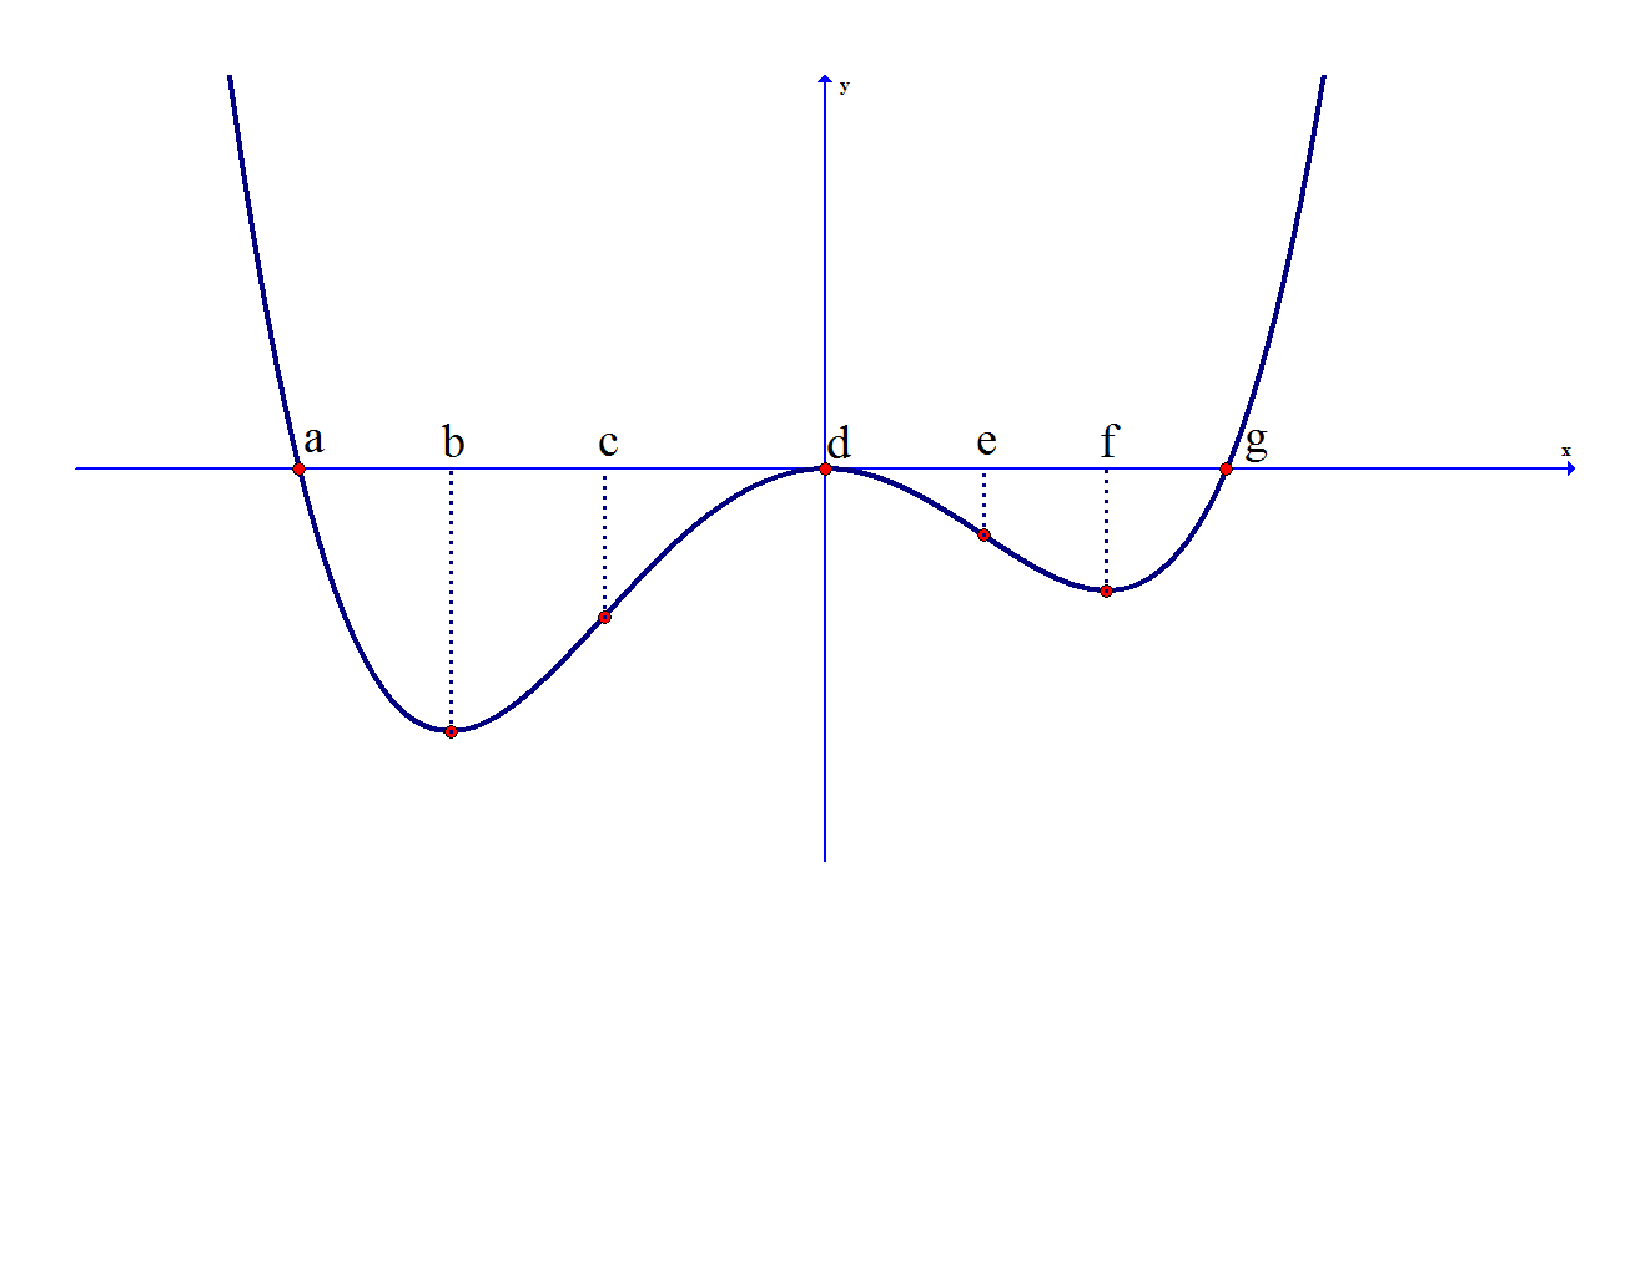
\includegraphics[scale=0.5]{graph.pdf}
\end{center}

\begin{enumerate}

\item Determine the interval(s) where $f(x)$ is increasing.

\ifans{\fbox{$(b,d) \cup (f,\infty)$}} \fi

\item Determine the interval(s) where $f(x)$ is decreasing.

\ifans{\fbox{$(-\infty,b) \cup (d,f)$}} \fi

\item Determine the interval(s) where $f(x)$ is concave up.

\ifans{\fbox{$(-\infty,c) \cup (e,\infty)$}} \fi

\item Determine the interval(s) where $f(x)$ is concave down.

\ifans{\fbox{$(c,e)$}} \fi

\item Determine the value(s) of $x$ where $f(x)$ has relative (local) extrema.  Classify each as the location of a relative maximum or a relative minumum.

\ifans{\fbox{Relative max when $x=d$; Relative minima when $x=b$ and $x=f$}} \fi

\item Determine the value(s) of $x$ where $f(x)$ has an inflection point.

\ifans{\fbox{Point of Inflection when $x=c$ and $x=e$}} \fi

\end{enumerate}

\item The graph of \underline{\bf the derivative} of $y=f(x)$ is shown below.

\begin{center}
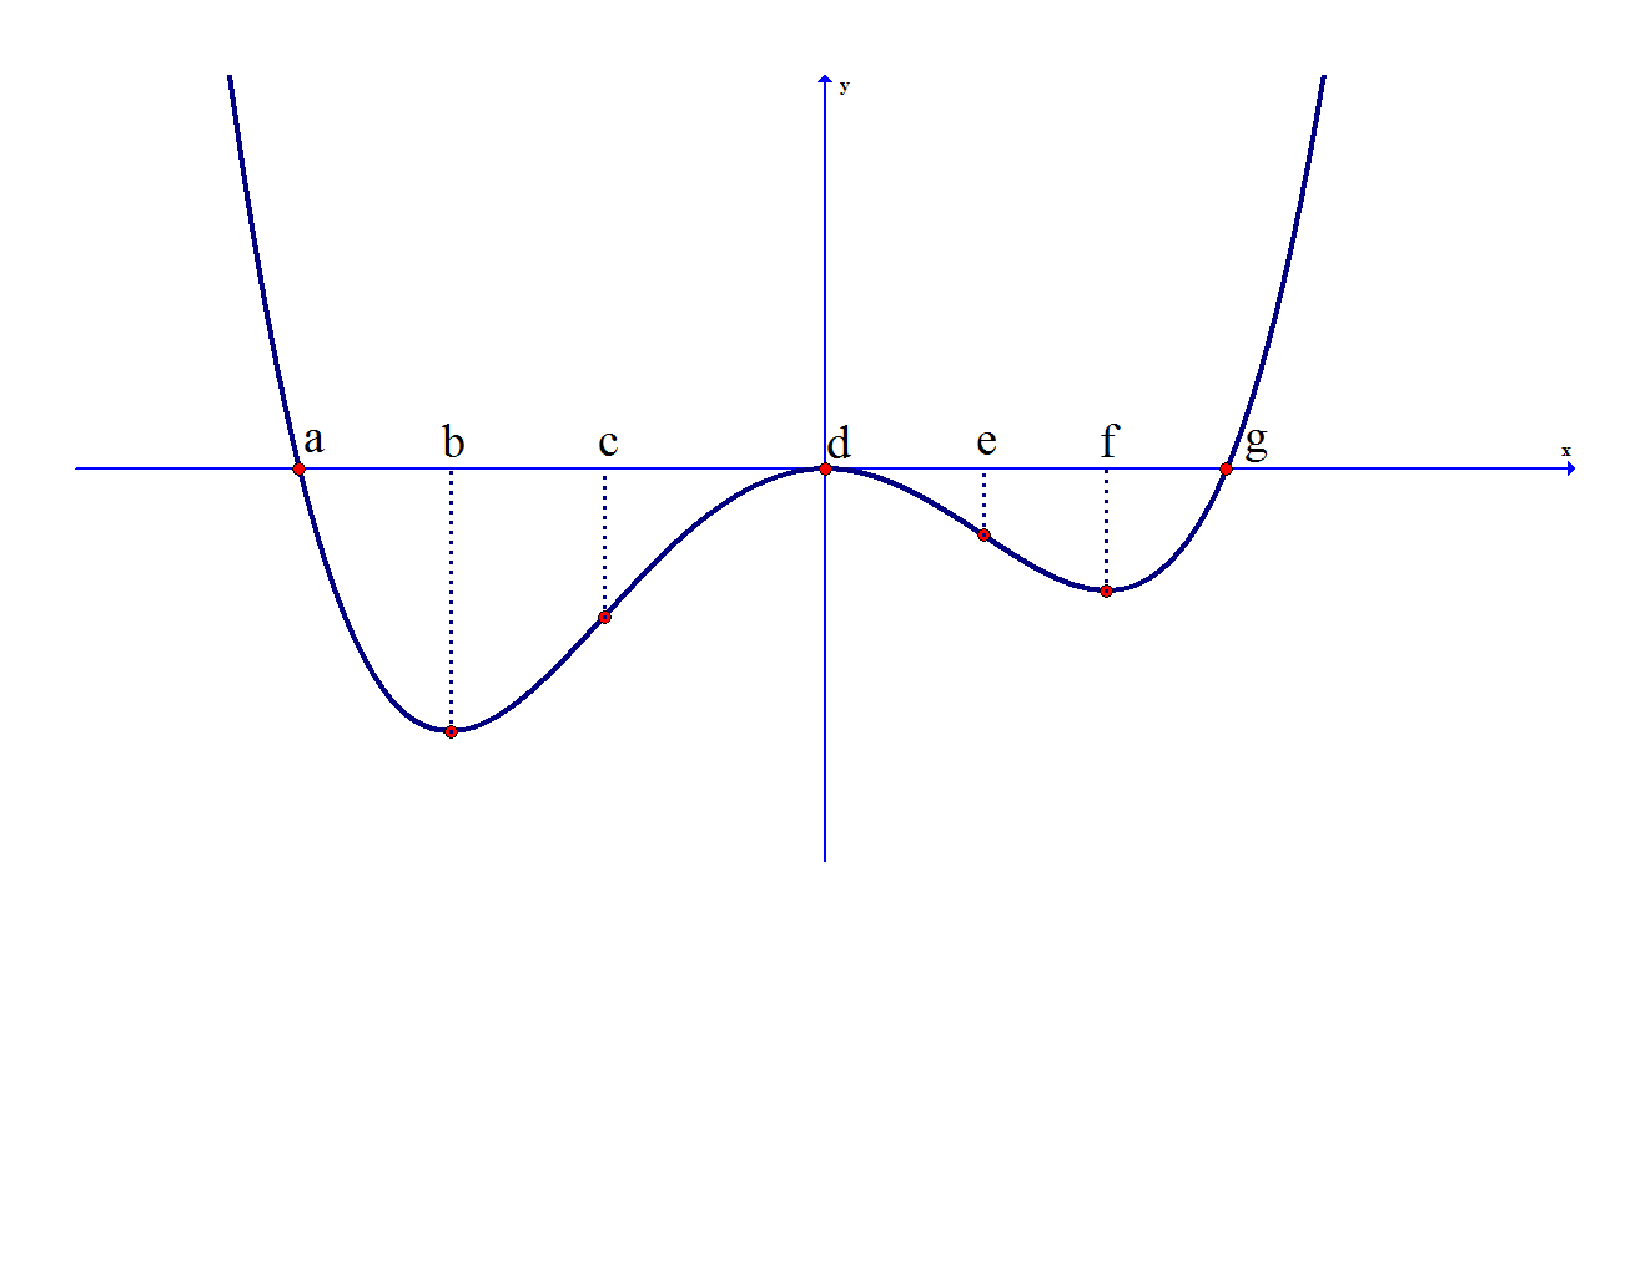
\includegraphics[scale=0.5]{graph.pdf}
\end{center}

\begin{enumerate}

\item Determine the interval(s) where $f(x)$ is increasing.

\ifans{\fbox{$(-\infty,a) \cup (g,\infty)$}} \fi

\item Determine the interval(s) where $f(x)$ is decreasing.

\ifans{\fbox{$(a,d) \cup (d,g)$}} \fi

\item Determine the interval(s) where $f(x)$ is concave up.

\ifans{\fbox{$(b,d) \cup (f,\infty)$}} \fi

\item Determine the interval(s) where $f(x)$ is concave down.

\ifans{\fbox{$(-\infty,b) \cup (d,f)$}} \fi

\item Determine the value(s) of $x$ where $f(x)$ has relative (local) extrema.  Classify each as the location of a relative maximum or a relative minumum.

\ifans{\fbox{\parbox{1\linewidth}{Relative maximum when $x=a$; Relative minimum when $x=g$; Neither a relative max nor a relative min at the critical point of $x=d$.}}} \fi

\item Determine the value(s) of $x$ where $f(x)$ has an inflection point.

\ifans{\fbox{Points of inflection when $x=b$, $x=d$ and $x=f$}} \fi

\end{enumerate}

\item Sketch the graph of a continuous function, $y=f(x)$, which is decreasing on $(-\infty,\infty)$, has an inflection point at $x=1$, and is concave down on $(1,\infty)$.

\ifans{\fbox{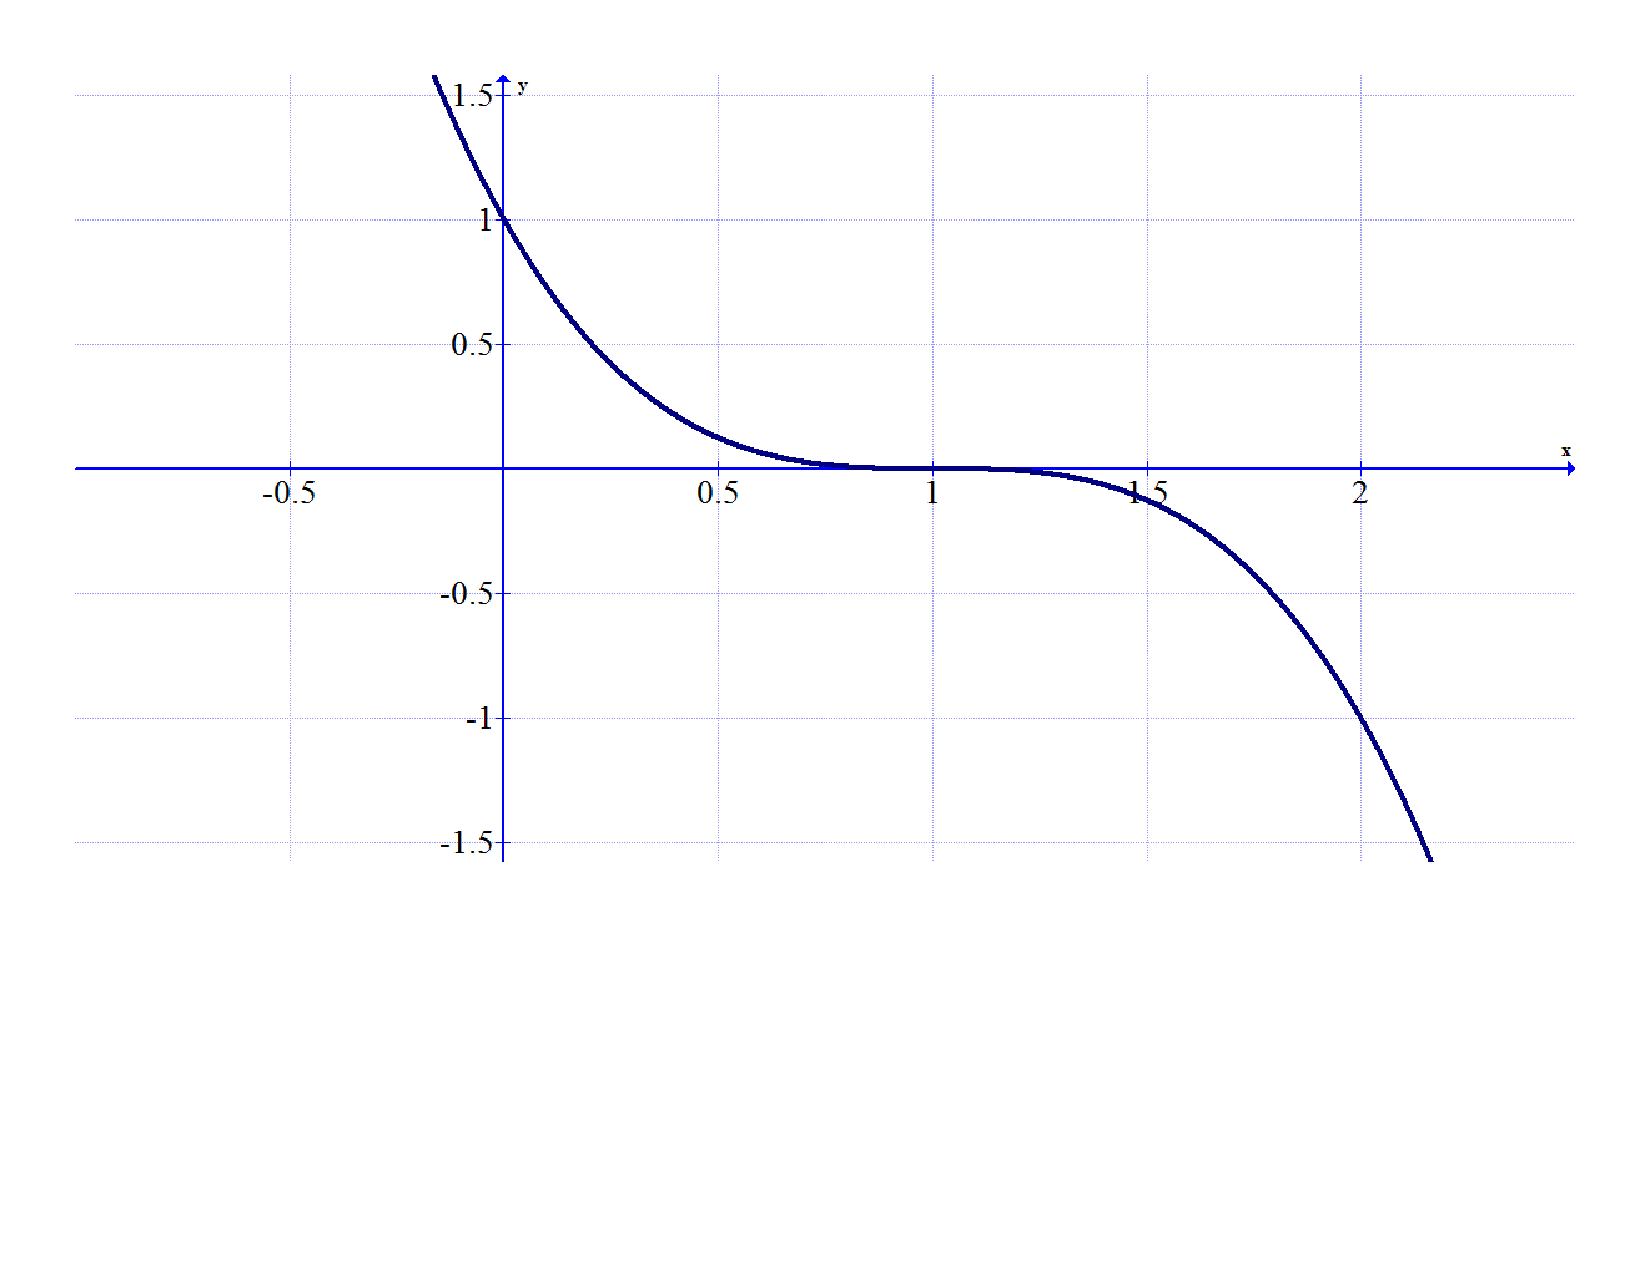
\includegraphics[scale=0.25]{graph1.pdf}}} \fi

\item Sketch the graph of a continuous function, $y=f(x)$, which is decreasing on $(-\infty,1)$, has a relative minimum at $x=1$, and does not have any inflection points.

\ifans{\fbox{\begin{tabular}{ccc}
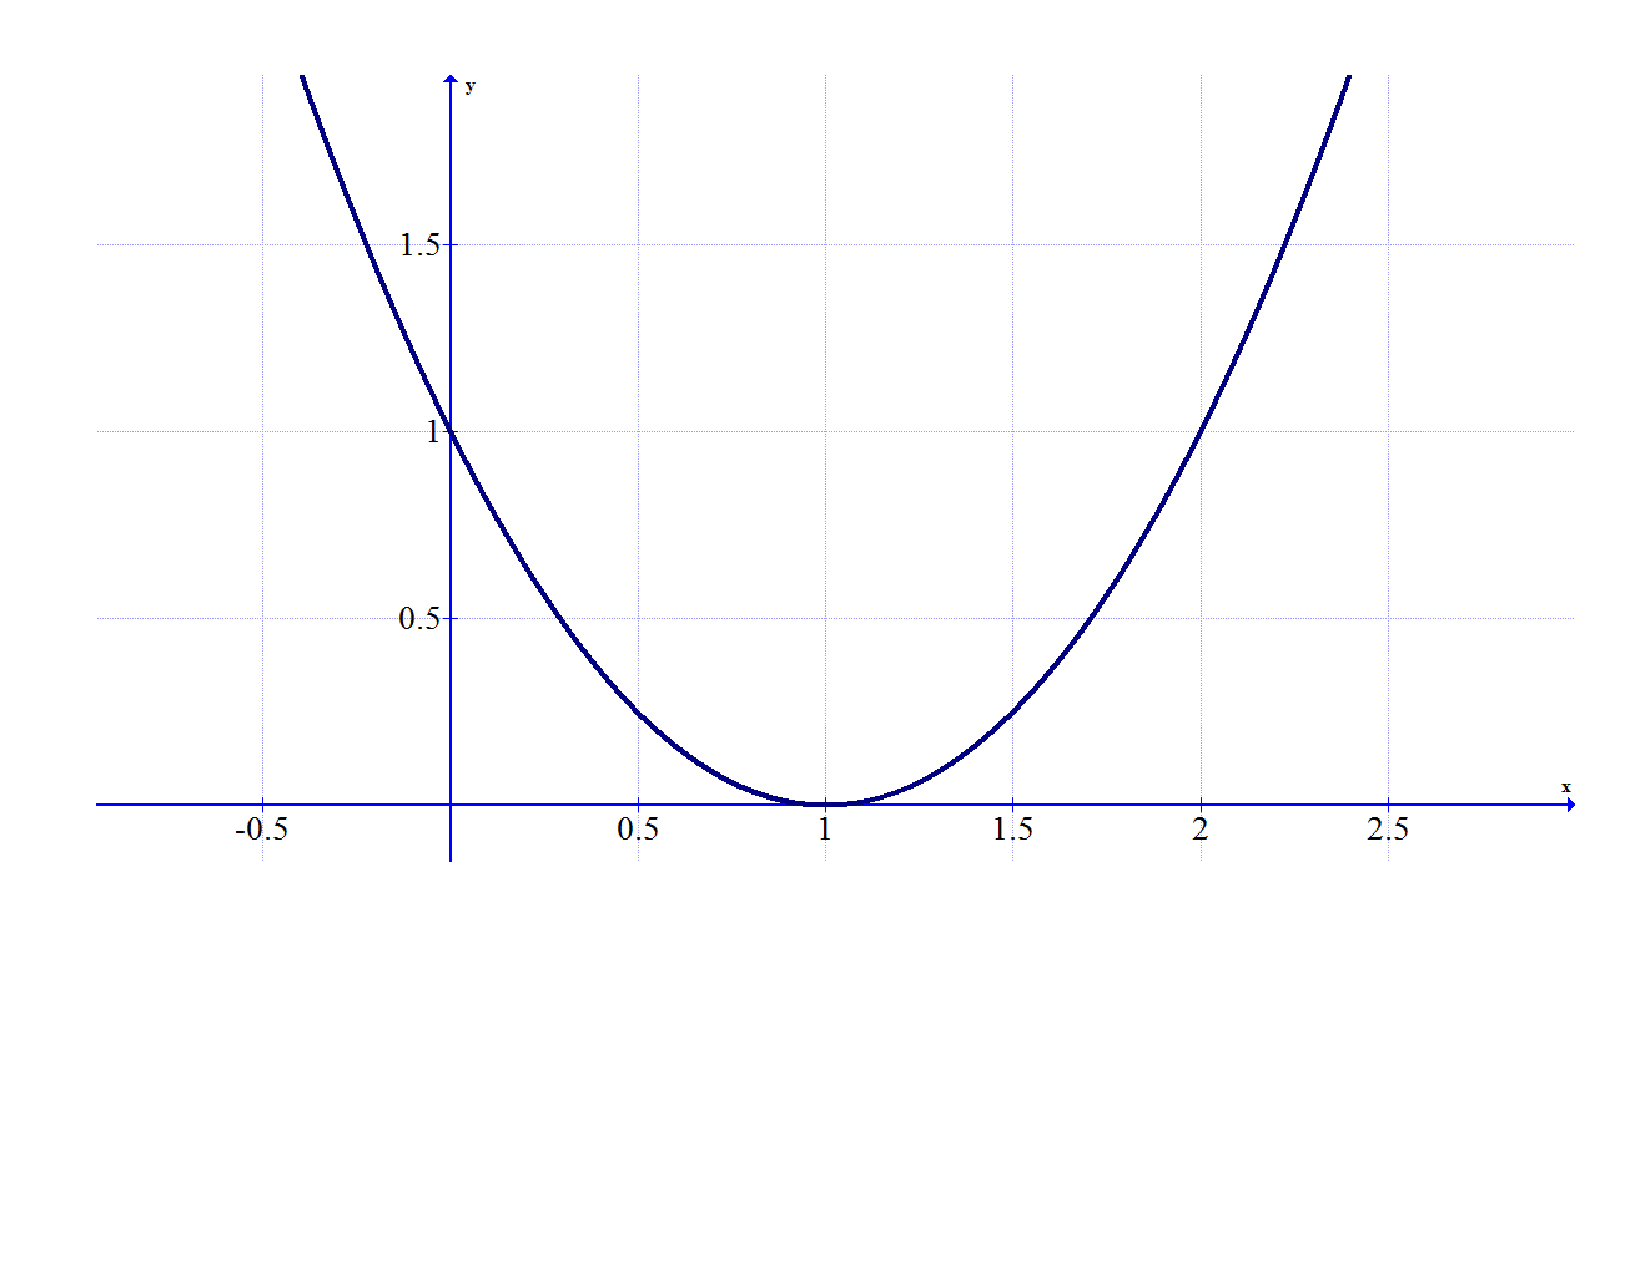
\includegraphics[scale=0.25]{graph2a.pdf} & or & 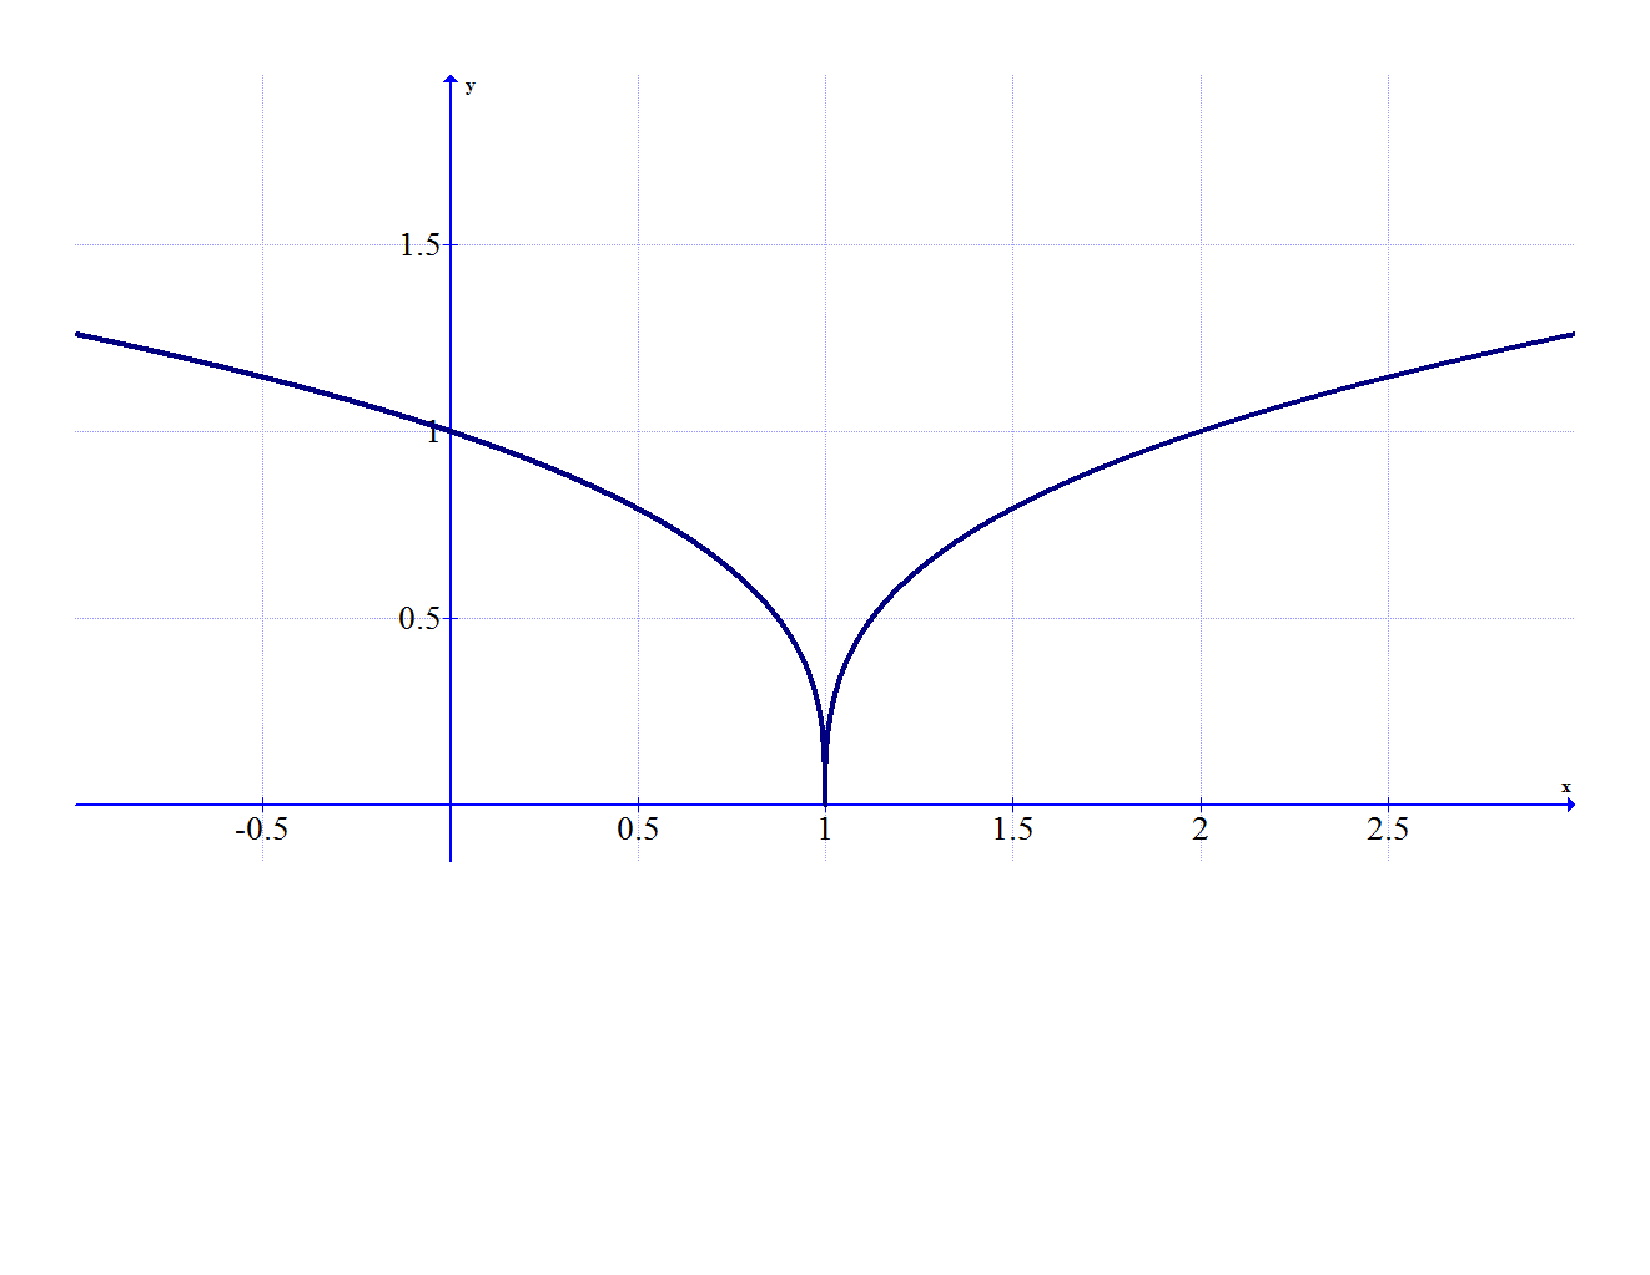
\includegraphics[scale=0.25]{graph2b.pdf}
\end{tabular}
}} \fi

\item Sketch the graph of a continuous function $y=f(x)$ which satisfies all of the following conditions:

\begin{itemize}

\item Domain of $f(x)$ is $(-\infty,\infty)$

\item $f(-1)=-2$, $f(0)=f(7)=3$, and $f(5)=9$

\item $f^{\prime}(x)<0$ on $(-\infty,-1) \cup (5,7)$ and $f^{\prime}(x)>0$ on $(-1,0)\cup (0,5) \cup (7,\infty)$

\item $f^{\prime \prime}(x)<0$ on $(0,7) \cup (7,\infty)$ and $f^{\prime \prime}(x)>0$ on $(-\infty,0)$

\end{itemize}

\ifans{\fbox{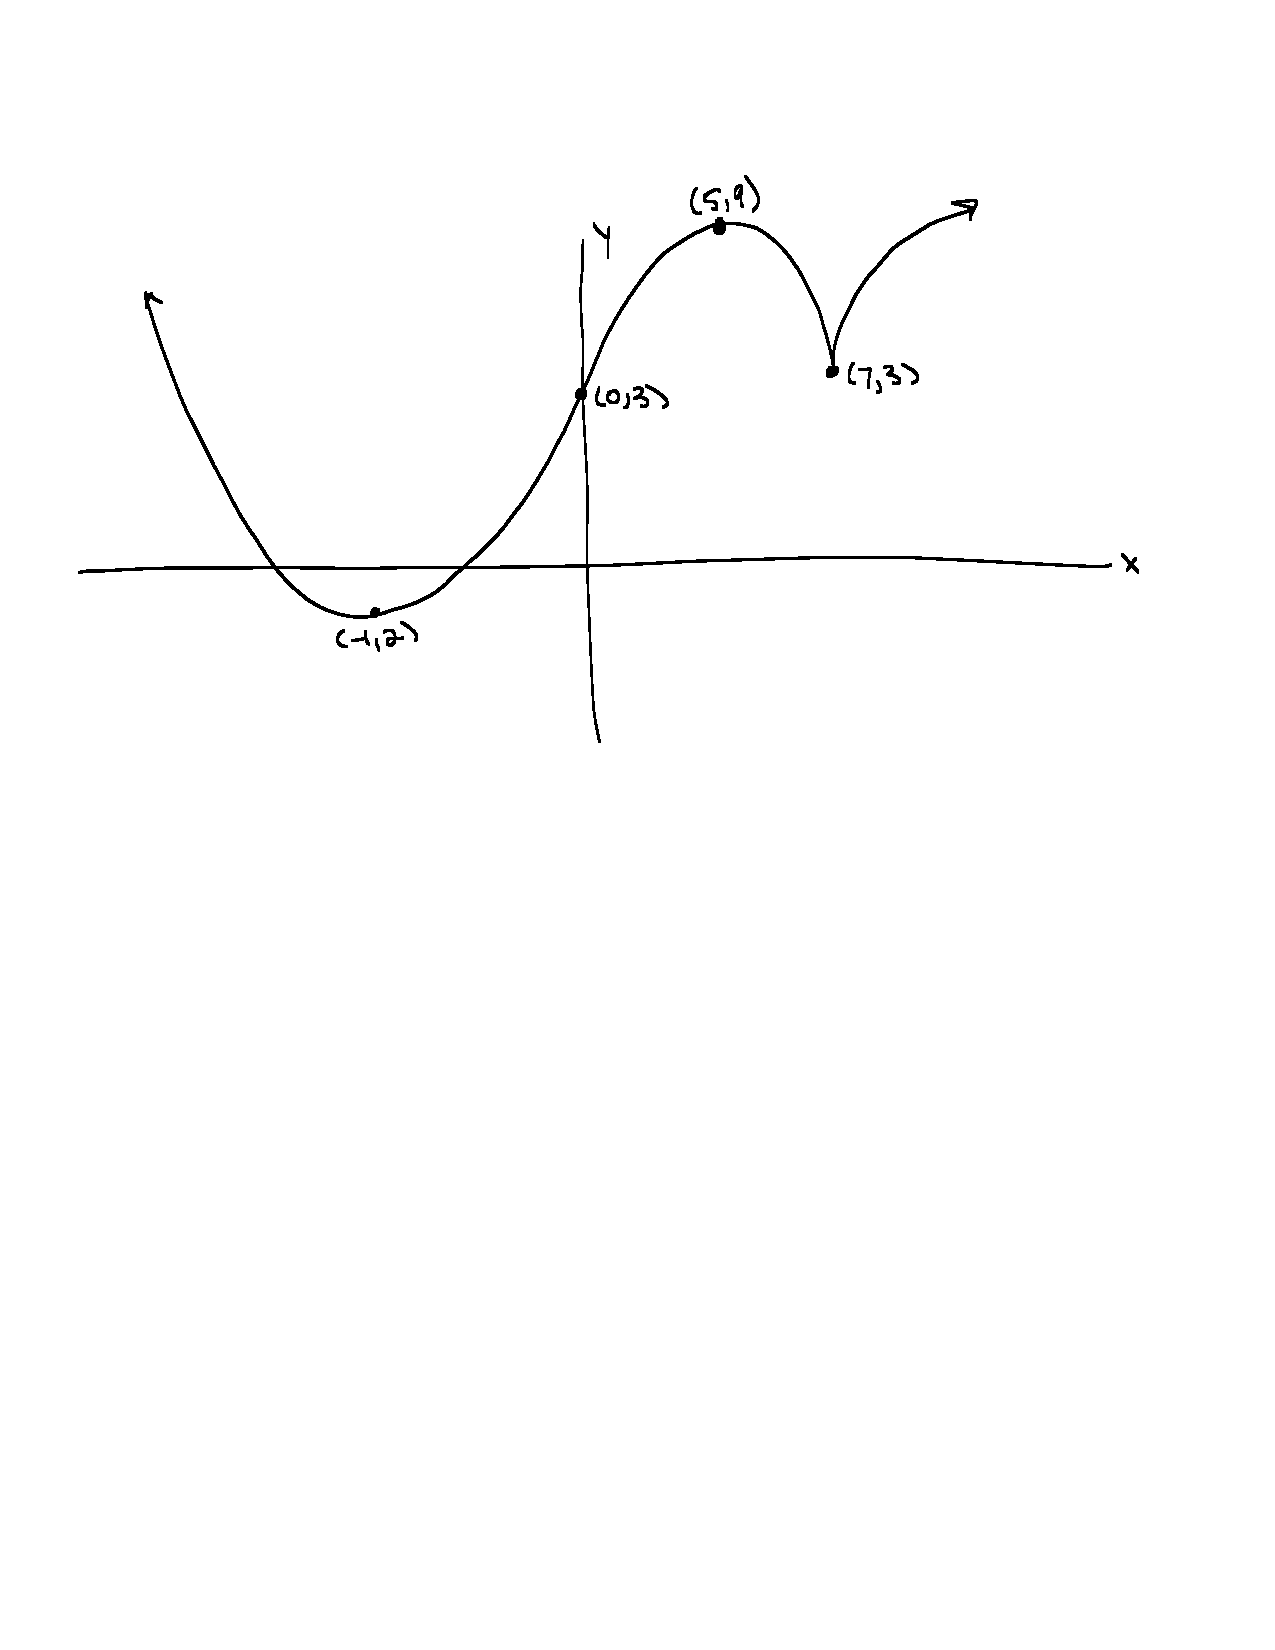
\includegraphics[scale=0.4]{graph3.pdf}}} \fi

\item Consider the function that you sketched in question 5.  At which value(s) of $x$ must $f^{\prime}(x)=0$?  At which value(s) of $x$ must $f^{\prime}(x)$ fail to exist?

\ifans{\fbox{$f^{\prime}(x)=0$ when $x=-1$ and $x=5$; $f^{\prime}(x)$ DNE when $x=7$}} \fi

\end{enumerate}

\noindent {\bf For problems 7-15, calculate each of the following:}\\

\begin{tabular}{ll}
(a) & The intervals on which $f(x)$ is increasing\\
(b) & The intervals on which $f(x)$ is decreasing\\
(c) & The intervals on which $f(x)$ is concave up\\
(d) & The intervals on which $f(x)$ is concave down\\
(e) & All points of inflection.  Express each as an ordered pair $(x,y)$
\end{tabular}\\

\begin{enumerate}
\setcounter{enumi}{6}

\item $f(x) = x^3-2x+3$ 

\ifans{\fbox{a.$\left(-\infty, -\sqrt{\frac{2}{3}}\right)\cup \left(\sqrt{\frac{2}{3}}, \infty \right)$; b. $\left(-\sqrt{\frac{2}{3}},\sqrt{\frac{2}{3}}\right)$; c. $(0,\infty)$; d. $(-\infty,0)$; e. $(0,3)$}} \fi

\item $f(x) = \frac{x}{x-2}$ 

\ifans{\fbox{a. none; b. $(-\infty,2) \cup (2,\infty)$; c. $(2,\infty)$; d. $(-\infty, 2)$; e. none}} \fi

\item $f(x) = \sin{x} \text{ on } [0,2\pi]$ 

\ifans{\fbox{a. $\left[0, \frac{\pi}{2}\right)\cup \left(\frac{3\pi}{2},2\pi \right)$; b. $ \left(\frac{\pi}{2}, \frac{3\pi}{2} \right)$; c. $(\pi, 2\pi)$; d. $(0,\pi)$; e. $(\pi,0)$}} \fi

\item $f(x) = (4x-1)^4$ 

\ifans{\fbox{a.$\left(\frac{1}{4},\infty \right)$; b. $\left(-\infty, \frac{1}{4}\right)$; c. $\left(-\infty,\frac{1}{4}\right) \cup \left(\frac{1}{4},\infty \right)$; d. none; e. none}} \fi

\item $f(x) = xe^x$ 

\ifans{\fbox{a. $(-1, \infty)$; b. $(-\infty, -1)$; c. $(-2,\infty)$; d. $(-\infty, -2)$; e. $\left(-2,-\frac{2}{e^2}\right)$}} \fi

\item $f(x) = \arctan{(2x)}$ 

\ifans{\fbox{a. $(-\infty,\infty)$; b. none; c. $(-\infty,0)$; d. $(0,\infty)$; e. $(0,0)$}} \fi

\item $f(x)=\frac{1}{\sqrt{2\pi}}e^{-x^2/2}$

\ifans{\fbox{a. $(-\infty,0)$; b.$(0,\infty)$; c. $(-\infty,-1) \cup (1,\infty)$; d. $(-1,1)$; e. $\left(-1,\frac{1}{\sqrt{2\pi} e^{1/2}}\right)$ and $\left(1,\frac{1}{\sqrt{2\pi} e^{1/2}}\right)$}} \fi

\item $f(x)=\frac{\ln{x}}{x}$

\ifans{\fbox{a. $(0,e)$; b. $(e,\infty)$; c. $(e^{3/2},\infty)$; d. $(0,e^{3/2})$; e. $\left(e^{3/2},\frac{3}{2e^{3/2}}\right)$}}\fi

\item $f(x)=2x+3x^{2/3}$

\ifans{\fbox{a. $(-\infty,-1) \cup (0,\infty)$; b. $(-1,0)$; c. none; d. $(-\infty,0) \cup (0,\infty)$; e. none}} \fi

\end{enumerate}

\noindent {\bf For problems 16-20, compute the critical points of the given function.  Then use the First Derivative Test to determine all relative (local) extrema.  Express each extremum as an ordered pair $(x,y)$.}

\begin{enumerate}
\setcounter{enumi}{15}

\item $f(x) = x^2-16$ 

\ifans{\fbox{Relative min at $(0,-16)$}} \fi

\item $f(x) = (2x+3)^3$ 

\ifans{\fbox{Critical Point at $-\frac{3}{2}$, No relative extrema}} \fi

\item $f(x) = \frac{3x}{x^2+1}$ 

\ifans{\fbox{Relative max at $\left(1,\frac{3}{2}\right)$; Relative min at $\left(-1,-\frac{3}{2}\right)$}} \fi

\item $f(x) = e^x-x$ 

\ifans{\fbox{Relative min at $(0,1)$}} \fi

\item $f(x) = x^3-x^5$ 

\ifans{\fbox{\parbox{1\linewidth}{
Relative maximum at $\left(\sqrt{\frac{3}{5}},\left(\frac{2}{5}\right) \cdot \left(\frac{3}{5}\right)^{3/2}\right)$\\
Relative minimum at $\left(-\sqrt{\frac{3}{5}},-\left(\frac{2}{5}\right) \cdot \left(\frac{3}{5}\right)^{3/2}\right)$\\
Critical point at $(0,0)$, which is neither a relative max nor a relative min}}} \fi

\end{enumerate}

\noindent {\bf For problems 21-22, use the Second Derivative Test to determine the relative (local) extrema.  Express each as an ordered pair $(x,y)$.}

\begin{enumerate}
\setcounter{enumi}{20}

\item $f(x) = \sin{(3x)}$ on $[0,\pi]$ 

\ifans{\fbox{Relative maxima at $\left(\frac{\pi}{6},1\right)$ and $\left(\frac{5\pi}{6},1\right)$; Relative minimum at $\left(\frac{\pi}{2},-1\right)$}} \fi

\item $f(x) = \sec{(3x)}$ on $[0,\pi]$ 

\ifans{\fbox{Relative minima at $(0,1)$ and $\left(\frac{2\pi}{3},1\right)$; Relative maxima at $\left(\frac{\pi}{3},-1\right)$ and $(\pi,-1)$}} \fi

\end{enumerate}

\noindent {\bf For problems 23-27, determine the critical points.  Classify each as a relative extremum, relative minimum, or neither.  Express all relative extrema as ordered pairs $(x,y)$.}

\begin{enumerate}
\setcounter{enumi}{22}

\item $f(x) = \sin^{2}{x} \text{ on } [0,2\pi]$ 

\ifans{\fbox{\parbox{0.55\linewidth}{
Relative minima at $(0,0)$, $(\pi,0)$, and $(2\pi,0)$;\\
Relative maxima at $\left(\frac{\pi}{2},1,\right)$ and $\left(\frac{3\pi}{2},1\right)$}}} \fi

\item $f(x)=\frac{x^3}{3}+x^2+x+3$

\ifans{\fbox{No relative extrema}} \fi

\item $f(x) = xe^x$  

\ifans{\fbox{Relative minimum at $\left(-1,-\frac{1}{e}\right)$}} \fi

\item $f(x)=2x+3x^{2/3}$

\ifans{\fbox{Relative maximum at $(-1,1)$; Relative minimum at $(0,0)$}} \fi

\item $f(x)=\frac{\ln{x}}{x}$

\ifans{\fbox{Relative Maximum at $\left(e,\frac{1}{e}\right)$}} \fi

\end{enumerate}

\noindent HINT: For problems 25-27, it may be helpful to use your work from earlier in the assignment.

\end{document}